\section{Observations}

In this section, we analyze the performance of the scheduling algorithms across different instances and configurations, focusing on the Relative Performance Ratio (RPR), the standard deviation of RPR, and the Relative Improvement when increasing the number of machines.

\subsection{Relative Performance Ratio}

The Relative Performance Ratio (RPR) is defined as the ratio of an algorithm's solution to the optimal solution, averaged over different seeds. Figure~\ref{fig:RPR-HEAT-G-A-m} presents a heatmap of the RPR for all combinations of generators and algorithms at $m = 2, 4, 6$ machines.

\begin{figure}
    \centering
    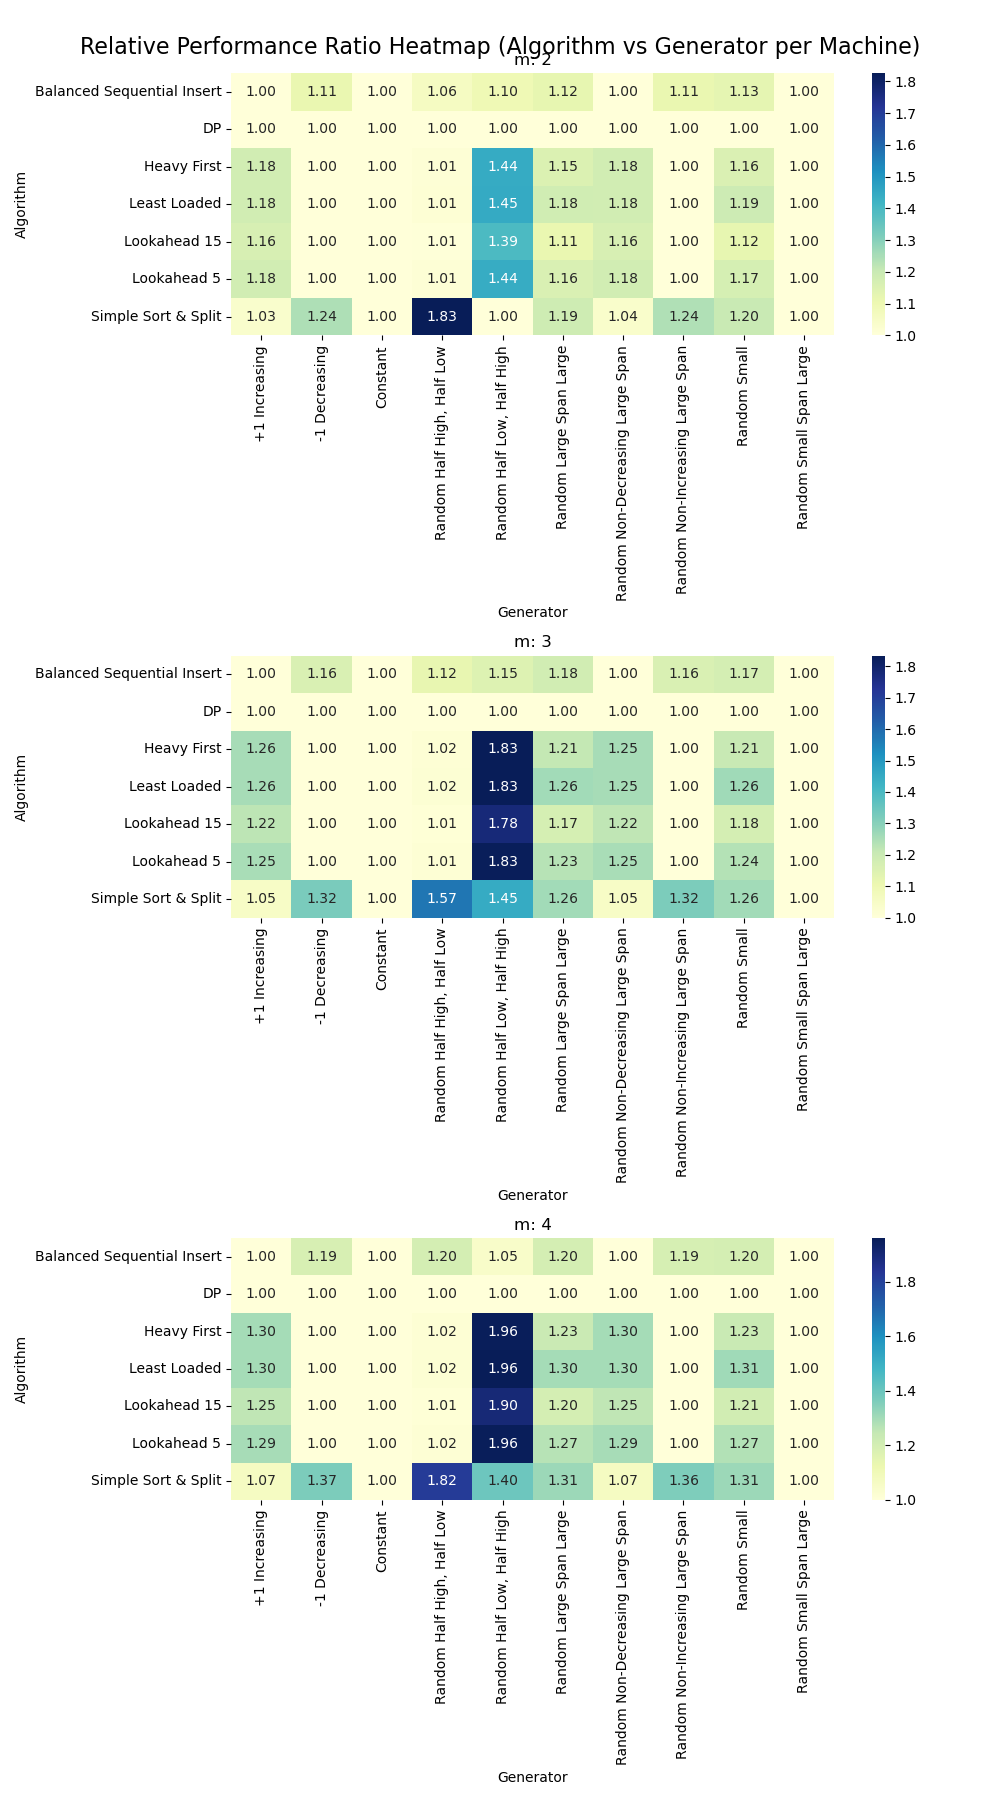
\includegraphics[height=.9\textheight]{RPR-HEAT-G-A-m.png}
    \caption{Relative Performance Ratio heatmap for all generators and algorithms at $m = 2, 4, 6$}
    \label{fig:RPR-HEAT-G-A-m}
\end{figure}

To facilitate analysis, we organized the generators and algorithms in a deliberate order, grouping similar ones together. For the generators, certain pairs exhibit equivalent behavior: \textit{Constant} and \textit{Random Small Span Large}, \textit{+1 Increasing} and \textit{Random Non-Decreasing Large Span}, \textit{$-1$ Decreasing} and \textit{Random Non-Increasing Large Span}, and \textit{Random Small} and \textit{Random Large Span Large}. Thus, we simplified the set of generators to six distinct types. The \textbf{Constant} generator represents trivial cases and is not examined further. The \textbf{Non-Increasing} category, originally \textit{$-1$ Decreasing} and \textit{Random Non-Increasing Large Span}, henceforth represented by \textit{$-1$ Decreasing}. Analogously, the \textbf{Non-Decreasing} category includes \textit{+1 Increasing} and \textit{Random Non-Decreasing Large Span}, represented by \textit{+1 Increasing}. The \textbf{Uniform Random} category, originally \textit{Random Small} and \textit{Random Large Span Large}, is represented by \textit{Random Small}; it is important that the maximum weight is several times greater than the minimum to avoid behavior similar to the \textit{Constant} generator. The \textbf{LoHi} and \textbf{HiLo} generators are originally named \textit{Half Low, then Half High} and \textit{Half High, then Half Low}, respectively.

For the algorithms, we observed that \textit{Least Loaded}, \textit{Heavy First}, \textit{Lookahead 5}, and \textit{Lookahead 15} perform very similarly, with \textit{Lookahead 15} having a slight edge. The \textit{Sort \& Split} algorithm generally underperforms compared to others, while the \textit{Balanced Sequential Insert (BSI)} algorithm maintains consistent performance as the number of machines increases and clearly outperforms \textit{Sort \& Split}. Therefore, we simplified the set of algorithms to four main categories: \textbf{Dynamic Programming (DP)} as the optimal solution, \textbf{Balanced Sequential Insert (BSI)}, \textbf{Sort \& Split (S\&S)}, and \textbf{Greedy}, which represents the group of algorithms originally called \textit{Least Loaded}, \textit{Heavy First}, \textit{Lookahead 5}, and \textit{Lookahead 15}.

Focusing on the \textit{Greedy}, \textit{BSI}, and \textit{S\&S} algorithms with the simplified set of generators, Figure~\ref{fig:RPR-LINE-G-A-m-INTERESTING} shows the RPR for these algorithms at $m = 3, 4, 5$.

\begin{figure}
    \centering
    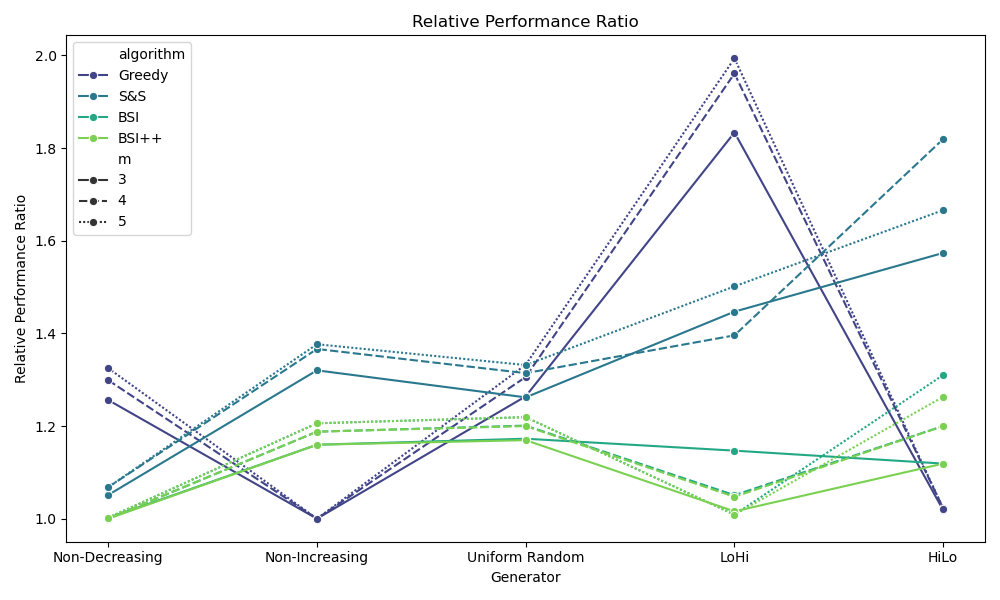
\includegraphics[width=\textwidth]{RPR-LINE-G-A-m-INTERESTING.png}
    \caption{Relative Performance Ratio for selected algorithms and generators at $m = 3, 4, 5$}
    \label{fig:RPR-LINE-G-A-m-INTERESTING}
\end{figure}

From the figure, we observe that the \textit{BSI} algorithm generally outperforms the others, except for the \textit{Non-Increasing} and \textit{HiLo} generators, where the \textit{Greedy} algorithm performs better. In these instances, the weights are such that they benefit from being uniformly distributed across the machines, aligning with the behavior of the \textit{Greedy} algorithm. This suggests that combining the strengths of both \textit{BSI} and \textit{Greedy} algorithms could lead to near-optimal performance across different types of instances.

Figure~\ref{fig:RPR-HEAT-G-m-A-INTERESTING} provides a heatmap highlighting the strengths and weaknesses of each algorithm for the selected generators across a range of machines from $m = 2$ to $6$.

\begin{figure}
    \centering
    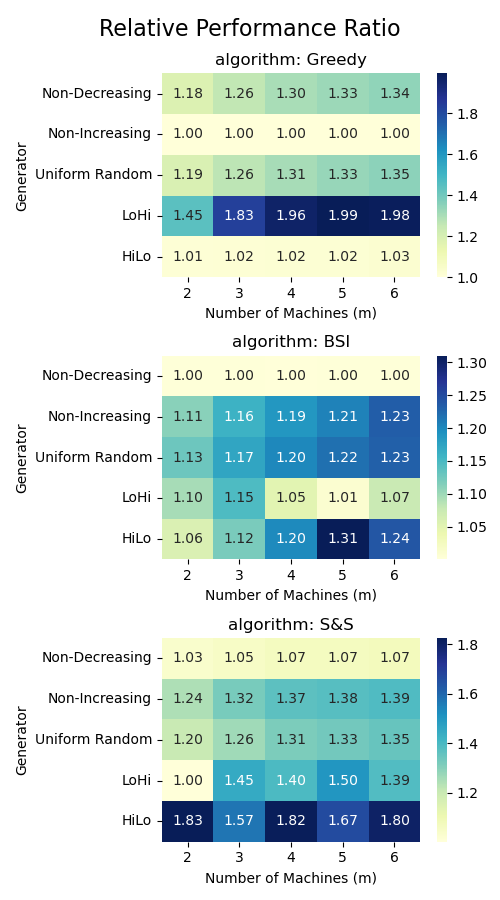
\includegraphics[width=0.6\textwidth]{RPR-HEAT-G-m-A-INTERESTING.png}
    \caption{Relative Performance Ratio heatmap for selected algorithms and generators across $m = 2$ to $6$}
    \label{fig:RPR-HEAT-G-m-A-INTERESTING}
\end{figure}

The \textit{Greedy} algorithm exhibits three distinct performance groups. It performs very well on the \textit{Non-Increasing} and \textit{HiLo} generators, with RPR in the range [1.0, 1.02]. On the \textit{Non-Decreasing} and \textit{Uniform Random} generators, its performance is poor, with RPR in the range [1.18, 1.35]. The algorithm performs very poorly on the \textit{LoHi} generator, with RPR ranging from 1.45 to 1.98.

The \textit{BSI} algorithm shows relatively stable performance across generators and machine counts. It performs very well on the \textit{Non-Decreasing} generator, with an RPR around 1.0. On the \textit{LoHi} generator, it performs well, with RPR between 1.01 and 1.15. For the \textit{Non-Increasing} and \textit{Uniform Random} generators, it achieves mediocre performance, with RPR between 1.11 and 1.23. However, its performance fluctuates on the \textit{HiLo} generator, with RPR ranging from 1.06 to 1.31.

The \textit{Sort \& Split} algorithm performs poorly to very poorly across the board, showing acceptable performance only with the \textit{Non-Decreasing} generator. These observations reinforce the potential benefit of combining the \textit{Greedy} and \textit{BSI} algorithms to exploit their respective strengths. By selecting the appropriate algorithm based on the instance characteristics, we can achieve near-optimal performance across different generators. Together, they provide very good performance on the \textit{Non-Increasing}, \textit{Non-Decreasing}, and \textit{HiLo} generators, with RPR between 1.0 and 1.02; good performance on the \textit{LoHi} generator, with RPR between 1.01 and 1.15; and mediocre performance on the \textit{Uniform Random} generator, with RPR between 1.11 and 1.23.

\subsection{Standard Deviation of RPR}

We examined the standard deviation of the RPR over different seeds to assess the stability of the algorithms. Figure~\ref{fig:RPR-STD-BAR-G-A} displays a bar chart of the standard deviation for all randomized generators and algorithms (excluding \textit{DP}) at $m = 5$.

\begin{figure}
    \centering
    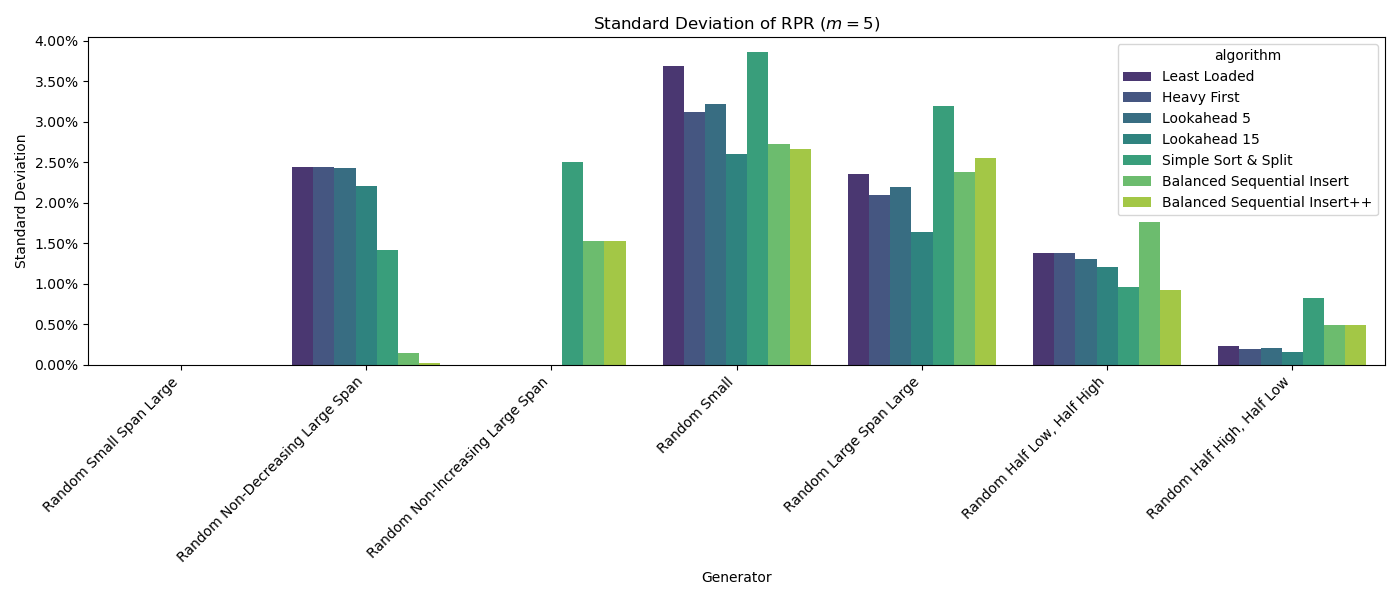
\includegraphics[width=\textwidth]{RPR_STD-BAR-G-A.png}
    \caption{Standard deviation of Relative Performance Ratio over seeds for randomized generators at $m = 5$}
    \label{fig:RPR-STD-BAR-G-A}
\end{figure}

Overall, the standard deviations are relatively low, less than $4\%$, indicating consistent performance across different seeds. The \textit{Uniform Random} generators exhibit the highest variability. The standard deviation is largely indifferent to the number of machines $m$, showing minimal differences. While this variability is acceptable in the current context, it could become problematic at larger scales, suggesting an area for future work.

\subsection{Relative Improvement}

We analyzed the Relative Improvement in the solution when increasing the number of machines from $m-1$ to $m$, defined as the percentage reduction in the solution value. Figure~\ref{fig:RI-LINE-A-m} illustrates the Relative Improvement for all algorithms (excluding \textit{DP}), averaged over randomized generators and seeds, across $m = 2, 3, 4, 6$.

\begin{figure}
    \centering
    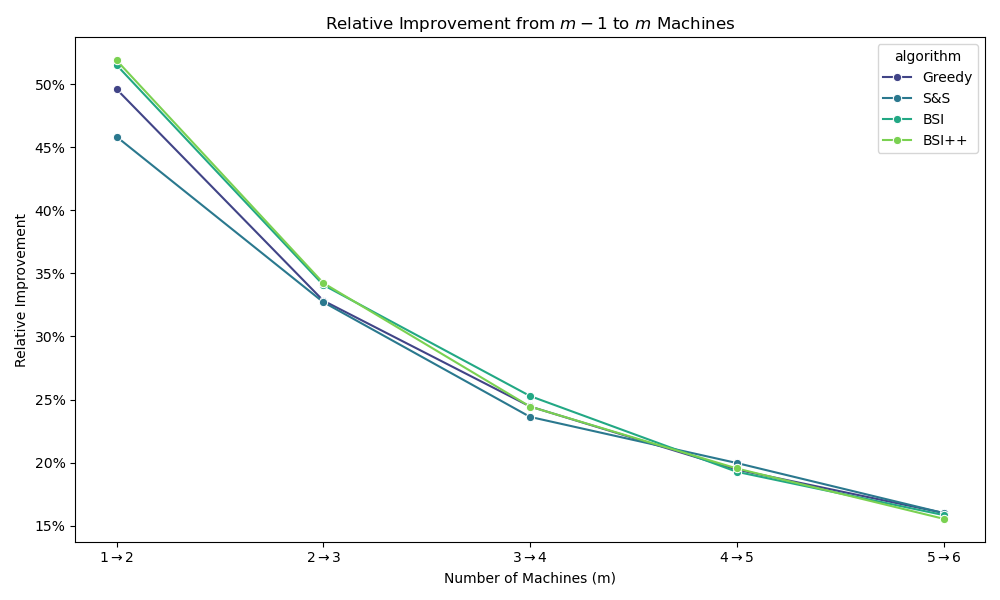
\includegraphics[width=\textwidth]{RI-LINE-A-m.png}
    \caption{Relative Improvement in solution quality when increasing the number of machines}
    \label{fig:RI-LINE-A-m}
\end{figure}

The results show no major differences among the algorithms, with all following a similar trend. This suggests that the algorithms neither asymptotically approach the optimal solution as the number of machines increases nor significantly diverge. Further investigation into asymptotic behavior over larger numbers of jobs ($n$) could provide additional insights.